\documentclass[10pt,aspectratio=169]{beamer}

% All the boilerplate is in ccaslides.sty
% Note that this also pulls in a custom vogtwidebar.sty
\usepackage{ccaslides}

\author{Ji\v{r}\'i Lebl}

\institute[OSU]{%
Departemento pri Matematiko de Oklahoma {\^S}tata Universitato}

\title{Cultivating Complex Analysis:\\%
Power series (2.3 part 1)}

\date{}

\begin{document}

\begin{frame}
\titlepage
\end{frame}

\begin{frame}
We will prove that holomorphic functions have power series, so let's study
power series.

\medskip
\pause

We first look at $z^n$. \pause
Locally, every power series and hence every holomorphic function looks like
$z^n$.

\medskip
\pause

$z^n$ is $n$-to-1 (except at $0$): 
\pause
For each $w = r e^{i\theta} \not=0$, there are $n$ distinct
$n$\textsuperscript{th} roots

\medskip
$\displaystyle
\qquad
r^{1/n} e^{i\theta/n}
, \quad
r^{1/n} e^{i\theta/n + 2\pi i /n}
, \quad \ldots, \quad
r^{1/n} e^{i\theta/n + 2\pi i (n-1)/n} .
$
\medskip
\pause

\vspace*{-0.2in}
\hspace*{3.5in}%
\subimport*{../figures/}{roots.pdf_t}


\vspace*{-0.9in}
They are equally
spaced out on a circle of radius $r^{1/n}$.

\medskip

e.g., in the picture $n=8$:

\medskip

$r^{1/8}$, $r^{1/8} e^{i \pi / 4}$,  $r^{1/8} e^{i \pi / 2}$,
etc.

\medskip
\pause


The roots of $w=1$ are
called the \emph{roots of unity}.
\end{frame}

\begin{frame}
If $z = re^{i\theta}$, then
\[
z^n = r^n e^{i n\theta} .
\]
It multiplies the angle by $n$.

\medskip
\pause
So $z^2$ takes sectors with vertex at the origin and doubles their angle.

\medskip
\pause

$z^2$ takes the sector
$\frac{-\pi}{2} \leq \Arg z \leq \frac{\pi}{2}$

to the closed right half-plane

$\{ z \in \C : \Re z \geq 0 \}$.

\vspace*{-0.7in}
\hspace{3in}%
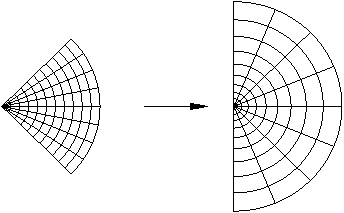
\includegraphics{../figures/zsqplot}

\pause
\vspace*{-0.1in}
It takes the first quadrant
$\{ z \in \C : \Re z \geq 0, \Im z \geq 0 \}$

to the closed upper half-plane $\{ z \in \C : \Im z \geq 0 \}$.

\medskip
\pause

It takes the second quadrant
$\{ z \in \C : \Re z \leq 0, \Im z \geq 0 \}$

to the closed lower half-plane $\{ z \in \C : \Im z \leq 0 \}$.

\medskip
\pause

Etc.
\end{frame}

\begin{frame}
The following useful statements about $z^n$ are left as an exercise:

\medskip
\pause

If $\sabs{z}<1$, then $\lim\limits_{n\to \infty} z^n = 0$.

\medskip
\pause

If $\sabs{z}>1$, then $\lim\limits_{n\to \infty} z^n = \infty$.

\medskip
\pause

If $z \not= 1$ is such that $\sabs{z}=1$, then $z^n$ diverges as $n \to
\infty$.
\end{frame}

\begin{frame}
A \emph{power series} around $p \in \C$ is
\[
\sum_{n=0}^\infty c_n {(z-p)}^n ,
\qquad \text{where } c_n \in \C.
\]
\pause

The series defines a function of $z$ (where it converges).

\medskip
\pause

It always converges (to $c_0$) if $z=p$.

\medskip
\pause

We say a power series is \emph{convergent} if
it converges for any $z \not= p$.
\end{frame}

\begin{frame}
The only power series we really honestly know how to sum is the:

\begin{proposition}[Geometric series]
\pause
\begin{enumerate}[(i)]
\item For $z \in \D$,
\quad
$\displaystyle
\frac{1}{1-z} = \sum_{n=0}^\infty z^n .
$
\pause
\item For $z \not\in \D$,
\quad
$\displaystyle
\sum_{n=0}^\infty z^n
$
diverges.
\pause
\item
Given $0 < r < 1$, then for all $z \in \overline{\Delta_r(0)}$,
\quad
$\displaystyle
\abs{\frac{1}{1-z} - \sum_{n=0}^m z^n}
\leq \frac{r^{m+1}}{1-r} .
$
\pause

Consequently,
as $\frac{r^{m+1}}{1-r} \to 0$,
the geometric series converges uniformly
on $\overline{\Delta_r(0)}$.
\end{enumerate}
\end{proposition}

\pause
\textbf{Proof:}
All three items follow (details an exercise) from
\[
1+z+z^2+\cdots+z^m = \frac{1-z^{m+1}}{1-z} ,
\qquad \text{for all } z \not= 1,
\]
\pause
which follows by expanding $(1-z)(1+z+z^2+\cdots+z^m)$.
\qed
\end{frame}

\begin{frame}
A power series \emph{converges absolutely} if
\[
\sum_{n=0}^\infty \sabs{c_n} \sabs{z-p}^n \quad \text{converges.}
\]
\pause
For $N < M$,
\[
\abs{\sum_{n=N+1}^M c_n {(z-p)}^n}
\leq
\sum_{n=N+1}^M \sabs{c_n} \sabs{z-p}^n .
\]
\pause
Hence,
if the sequence of partial sums of 
$\sum \sabs{c_n} \sabs{z-p}^n$ is Cauchy,

so is the sequence
of partial sums of $\sum c_n {(z-p)}^n$.

\medskip
\pause
Thus, an absolutely convergent series converges.
\end{frame}

\end{document}
